\documentclass{standalone}
\usepackage{amssymb}
\usepackage{amsfonts}

\usepackage{unicode-math}
\usepackage{fontspec}
\usepackage{tikz,pgfplots}


\usetikzlibrary{patterns}

\setmainfont{EB Garamond}[Ligatures=Rare]
\setmathfont{Garamond-Math.otf}[StylisticSet={2, 7, 9}]
\setmathfont{Garamond-Math.otf}[StylisticSet={2, 7, 9, 8}, version=a]


\everymath{\displaystyle}
\begin{document}

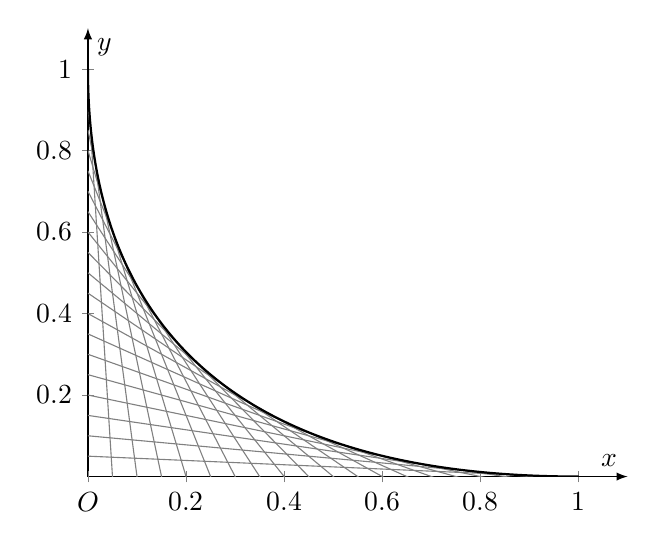
\begin{tikzpicture}
    \begin{axis}[
            axis x line=middle,
            axis y line=middle,
            every inner x axis line/.append style={-latex},
            every inner y axis line/.append style={-latex},
            legend pos = north west,
            xlabel=$x$,
            ylabel=$y$,
            ymajorgrids=false,
            xmajorgrids=false,
            grid style=dashed,
            ymax=1.1,ymin=0,
            xmax=1.1,xmin=0,
            extra x ticks={0},
            extra x tick labels={\(O\)},
        ]
        \foreach \i in {1,2,...,19}{
                \addplot[
                    color=gray,domain=0:1,
                ]
                {\i/20+ (x*\i)/(\i-20)}
                %\closedcycle
                ;
            }
        \addplot[
            color=black, samples=10000,thick,domain=0:1,
        ]
        {(1-x^(0.5))^2}
        ;
    \end{axis}
\end{tikzpicture}

\end{document}